\subsubsection{Luftflöde genom väggar – drag}

\begin{figure}
\centering
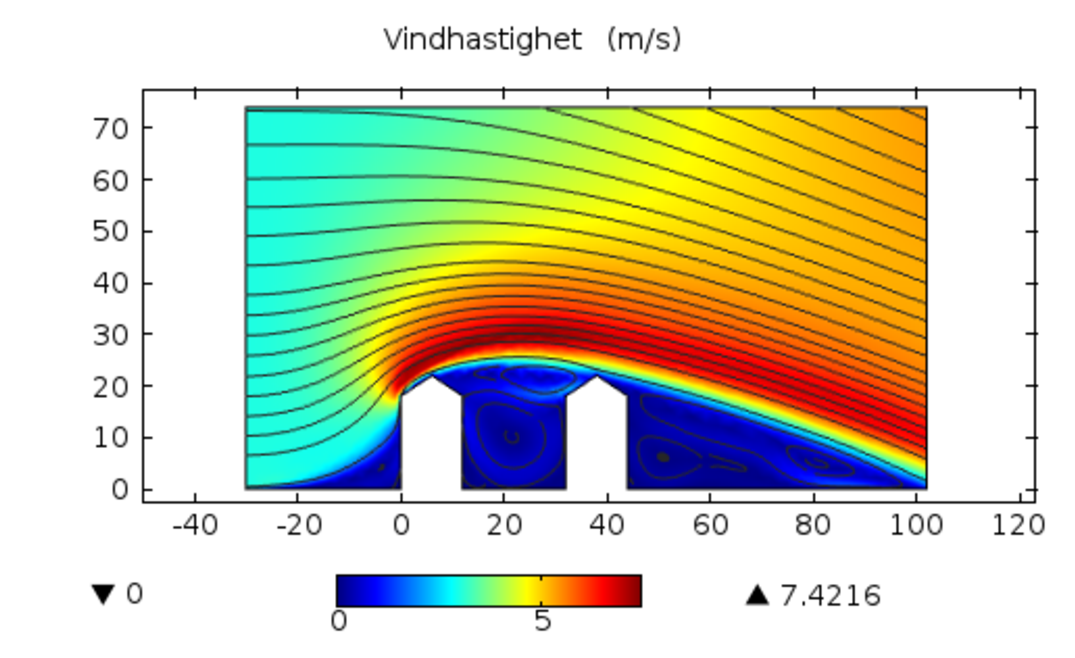
\includegraphics[width=130mm,height=78mm]{images/wind3ms.eps}
\caption{Vindhastiheten när vind i $\unit[3]{ m/s}$ blåser mot fastigheten. Linjerna
i figuren är strömlinjer och färgen indikerar beloppet av hastighetsvektorn. Värdena är framräknade med Comsol.}
\end{figure}

\begin{figure}
\centering
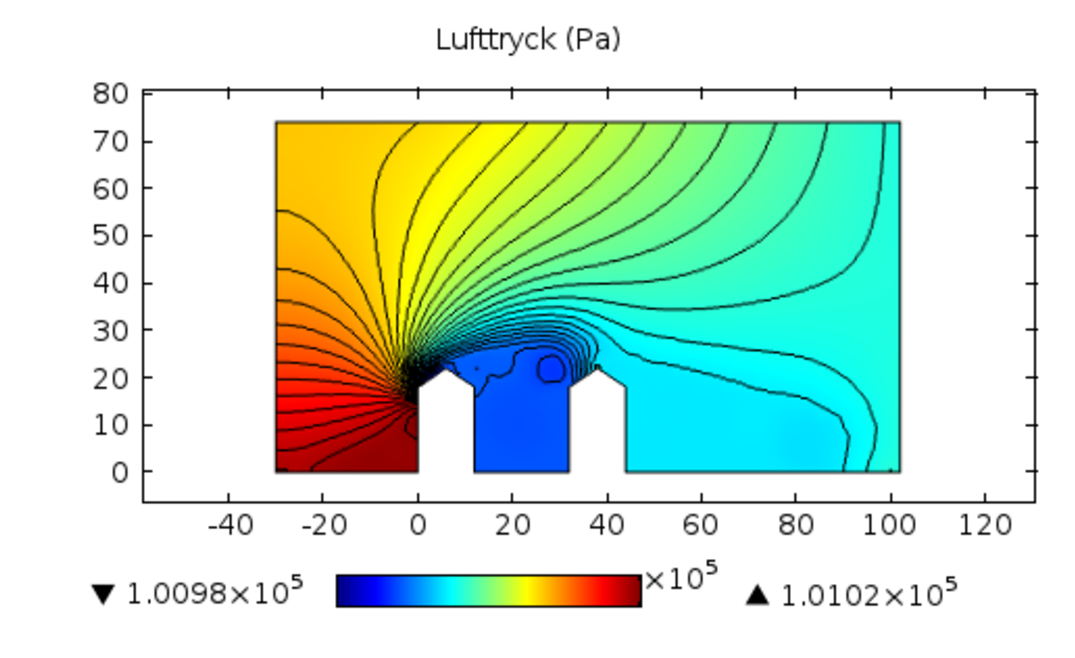
\includegraphics[width=130mm,height=78mm]{images/pressure3ms.eps}
\caption{Lufttrycket när vind i $\unit[3]{ m/s}$ blåser från vänster
sida i figuren. Färgen indikerar lufttryck och linjer ligger längs isobarer.
Tryckskillnaderna på de olika sidorna av husen kommer att driva ofrivillig ventilation vilket leder till infiltrationsförluster.}
\end{figure}
